\documentclass[../cnd.tex]{subfiles}
\subsubsection{Đào mỏ}
Do một hệ thống phân phối không có chủ sở hữu duy nhất, các máy có thể được tự do tham gia các mạng Ethereum theo ý thích và bắt đầu xác nhận giao dịch. Quá trình này được gọi là đào mỏ.

Việc đào mỏ đi đến một sự đồng thuận về thứ tự của các giao dịch trên toàn hệ thống, điều này là cần thiết để lập bảng cân đối tài khoản của tất cả mọi người một cách nhanh chóng, ngay cả khi nhiều giao dịch thông qua mạng. Quá trình này tiêu thụ điện năng, đó là chi phí tiền bạc, và vì vậy người thợ mỏ được trả một phần thưởng cho mỗi khối họ khai thác: khoảng 5 ether.

\subsubsection{Ether}
Tiền mã hóa được giao dịch trong mạng lưới Ethereum được gọi là ether. Nó được niêm yết dưới mã ETH và giao dịch trên các sàn giao dịch tiền mã hóa. Nó cũng được sử dụng để trả phí giao dịch và dịch vụ tính toán trên mạng Ethereum.

Đối với tiền ảo, thách thức để được chấp nhận vẫn còn tồn tại. Ngày nay, những tiền ảo này vẫn là một lớp thanh toán nhanh, bảo mật và minh bạch nhất trong các hệ thống tiền tệ đang tồn tại được công nhận; Sự triển khai thử nghiệm các đồng tiền ảo này một ngày nào đó có thể thay thế các công nghệ mạng thanh toán tập trung như Visa hay Mastercard ngày nay.

\subsubsection{Gas}
Gas là một đơn vị được sử dụng để đo lường mức chi phí tính toán (computationally expensive) có thể tiêu tốn cho một giao dịch trên Ethereum. Giá trị của gas được quy đổi bằng một lượng ether tương ứng.

Nói cách khác gas không phải là một đơn vị tiền tệ, và bạn không thể sở hữu hay tích trữ nó. Nó chỉ đơn giản đo đạc mức tiêu hao của các phép tính toán mà hệ thống phải chịu nếu thực hiện giao dịch. Để có thể trả chi phí gas, bạn chỉ cần thêm ether vào tài khoản của bạn. Mọi toán tử trên EVM đều có một giá trị gas nhất định.

Có hai lý do chính để gas ra đời:
\begin{itemize}
	\item Thứ nhất, nó là một phần thưởng đảm bảo được đặc tả trước cho các thợ đào (miner) trong việc thực thi mã nguồn và bảo mật kết mạng, ngay cả khi việc thực thi bị thất bại vì một lý do nào đó. 
	\item Thứ hai, nó đảm bảo việc thực thi không thể dài quá thời gian đã được ước lượng trước đó.
\end{itemize}

Việc này khác so với Bitcoin, nơi mà chi phí được tính bằng kích thước của giao dịch (tính bằng kilobytes), ta có thể thấy việc tính chi phí dựa trên khối lượng tính toán hợp lý hơn nhiều.

Hệ thống gas cũng không khác lắm so với việc đo lượng điện dân dụng. Điểm khác biệt với thị trường năng lượng thực chính là người tạo giao dịch sẽ quyết định giá gas (thợ mỏ có thể chấp nhận giá này hoặc không)

Giá gas cho mỗi giao dịch hay hợp đồng được thiết lập để xử lý bản chất Turing Complete của Ethereum và EVM của nó (tức là mã Ethereum Virtual Machine)- đây là một trong những ý tưởng được đưa ra để hạn chế vòng lặp vô hạn. Ví dụ như 10 szabo, tương đương với 0.00001 ether hay 1 gas có thể thực hiện một dòng mã hay vài câu lệnh. Nếu không có đủ ether trong tài khoản để hiển thị một cuộc giao dịch hay một tin nhắn thì nó được coi là không hợp lệ. Ý tưởng này sẽ phần nào ngăn chặn được những cuộc tấn công từ vòng lặp vô hạn, khuyến khích tính hiệu quả trong chuỗi mã - và bắt những kẻ tấn công phải trả cho tài nguyên mà mình sử dụng. Câu lệnh càng phức tạp thì bạn càng phải trả nhiều gas hơn.
\begin{figure}[ht]
	\centering
	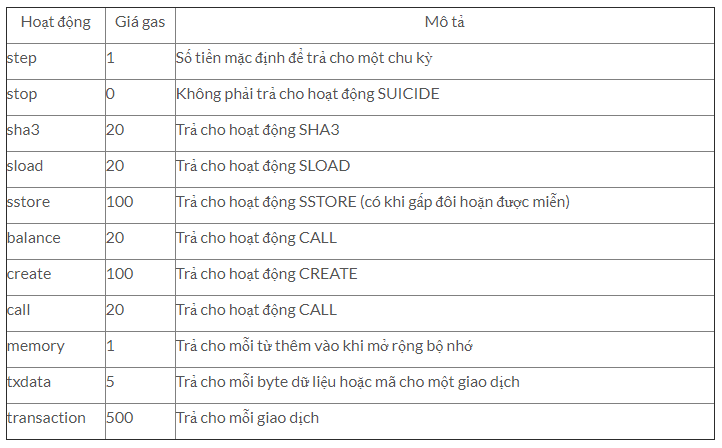
\includegraphics[width=0.85\linewidth]{../img/gasPrice}
	\caption{Danh sách các hoạt động trong Ethereum Virtual Code 
		\\ và giá của nó (tính theo Gas)$^{[8]}$}
	\label{fig:gasprice}
\end{figure}

\subsubsection{Máy ảo Ethereum}
Máy ảo Ethereum (Ethereum Virtual Machines, viết tắt là EVM) là một máy chủ toàn cầu mà mọi người có thể sử dụng với một chi phí nhỏ, có thể trả bằng ether.

\paragraph{Mạng ngân hàng trung tâm}\mbox{}\\

Chúng ta đang chi rất nhiều tiền cho việc xây dựng, vận hành và bảo trì các hệ thống thanh toán tập trung. Mỗi ngân hàng xây dựng riêng cho mình một hệ thống và việc thanh toán liên ngân hàng sẽ đòi hỏi thêm một khoản phí nữa, chưa kể đến các chi phí để đảm bảo an toàn, an ninh cũng như tính tin cậy cho cả hệ thống. Những chi phí ấy không hề rẻ dẫn đến việc bạn phải chi trả nhiều hơn cho các giao dịch của mình cũng như các giao dịch sẽ bị chậm đi đáng kể khi phải liên kết niều dịch vụ.

\paragraph{Máy ảo}\mbox{}\\

Trong ngữ cảnh của Ethereum, đó là một máy tính toàn cầu bao gồm rất nhiều nút cấu thành và chính các nút đó cũng là các máy tính. Nói chung, máy ảo là mô phỏng một hệ thống máy tính này bằng một hệ thống máy tính khác. Việc mô phỏng này trên EVM sử dụng cả phần cứng và phần mềm, mỗi nút trong mạng có thể chạy bất kì hệ điều hành nào.

\paragraph{Vai trò của EVM}\mbox{}\\

EVM tạo ra môi trường để chạy các chương trình bất kì (được gọi là các hợp đồng thông minh) được viết bằng ngôn ngữ Solidity. Những chương trình này là xác định đầy đủ và đảm bảo là được thực hiện nếu bạn trả đủ chi phí cho giao dịch.

Các chương trình viết bằng Solidity có khả năng thực hiện tất cả các nhiệm vụ có thể thực hiện được bằng máy tính. Khi một hợp đồng được triển khai bằng việc tải lên từ một nút của mạng, các bản sao của hợp đồng sẽ được phát tán ra các nút khác. Khi có yêu cầu chạy hợp đồng, các nút trong mạng sẽ chạy một các độc lớp với cùng một mã của hợp đồng. Tuy nó cho thấy sự song song hóa rất cao, nhưng nó cũng mang lại sự dư thừa không hề nhỏ.

EVM đã được lập trình trong C++, Go, Haskell, Java, Python, Ruby, Rust và WebAssembly (hiện đang được phát triển)

\subsubsection{Hợp đồng thông minh}
Bình thường, khi ký một hợp đồng để trao đổi giá trị kinh tế, chúng ta cần một bên thứ 3 có trách nhiệm hòa giải (ví dụ: Nhà môi giới, Tòa án, Sở đất đai,...). Hợp đồng thông minh (smart contract) là một cơ chế trao đổi xác định, được kiểm soát bởi các phương tiện kỹ thuật số mà có thể giúp cho việc thực hiện giao dịch trực tiếp giữa các thực thể mà không cần tin cậy nhau. Các hợp đồng này được định nghĩa bằng cách lập trình và được chạy chính xác như mong muốn mà không bị kiểm duyệt, lừa đảo hay sự can thiệp từ bên thứ ba trung gian.

Chúng có thể được sử dụng để tạo điều kiện, xác minh và thực thi việc đàm phán hoặc thực hiện các hướng dẫn thủ tục kinh tế và có khả năng tránh được sự kiểm duyệt, thông đồng và rủi ro từ phía đối tác. Trong Ethereum, các hợp đồng thông minh được coi là các kịch bản tự trị hoặc các ứng dụng phân cấp được lưu trữ trong chuỗi khối Ethereum để thực hiện sau đó bởi EVM. Các hướng dẫn được nhúng trong các hợp đồng Ethereum được thanh toán bằng ether và có thể được thực hiện bằng nhiều ngôn ngữ Turing hoàn chỉnh khác nhau.

Sự khác biệt giữa hợp đồng truyền thống và hợp đồng thông minh:
\begin{itemize}
	\item Hợp đồng truyền thống được tạo ra bởi các chuyên gia pháp lí để biên soạn và thi hành. Điều này rất mất thời gian và không minh bạch hoàn toàn. Khi có sự cố xảy ra thì phải dựa vào hệ thống pháp lí để giải quyết hợp đồng và điều này sẽ tốn các chi phí liên quan.
	\item Hợp đồng thông minh được tạo ra bởi hệ thống máy tính bằng ngôn ngữ lập trình. Trong đó nêu rõ các điều khoản và hình phạt tương đương với các hợp đồng truyền thống đưa ra. Nhưng hợp đồng thông minh không cần sự can thiệp của con người, do đó đảm bảo việc thực thi hợp đồng được chính xác và công minh nhất. Toàn bộ hợp đồng thông minh được thực hiện bởi hệ thống chuỗi khối phân tán.
\end{itemize}

\subsubsection{Tài khoản Ethereum}

Mỗi tài khoản Ethereum được đại diện bởi 20 ký tự. Các thông số sau được lưu trong dữ liệu trạng thái (state) của Ethereum cho mỗi tài khoản:
\begin{itemize}
	\item Số nonce: để đảm bảo mỗi giao dịch chỉ được xử lý một lần.
	\item Số dư tài khoản
	\item Mã nguồn hợp đồng (nếu có)
	\item Phần lưu trữ của tài khoản (mặc định là trống)
\end{itemize}
	
Các giao dịch giữa các tài khoản được trả tiền bằng ether. Có hai loại tài khoản: tài khoản ngoại vi được quản lý bởi khóa riêng tư, và tài khoản hợp đồng được quản lý bởi mã hợp đồng. Tài khoản ngoại vi không chứa mã hợp đồng, có thể gửi thông điệp đi bằng cách tạo và ký kết một giao dịch, giống như tài khoản Bitcoin. Về phía tài khoản hợp đồng, mỗi khi nó nhận được 1 thông điệp, mã hợp đồng sẽ chạy và cho phép đọc và ghi vào phần lưu trữ của nó, kèm theo việc gửi thông điệp đi và tạo ra hợp đồng khác lần lượt.

Lưu ý rằng "hợp đồng" trong Ethereum không phải là một cái gì đó phải "hoàn thành" (fulfilled) hoặc "tuân thủ" (complied with). Thay vào đó, nó giống như các "thực thể tự trị" sống bên trong môi trường Ethereum, luôn thực hiện một đoạn mã cụ thể khi được tác động bởi một thông điệp hoặc giao dịch, và có quyền kiểm soát trực tiếp số ether và dữ liệu trong phần lưu trữ của nó.

\subsubsection{Thông điệp và giao dịch}
Thuật ngữ "giao dịch" được sử dụng để chỉ tới gói dữ liệu mà bao gồm thông điệp. Một giao dịch bao gồm:
\begin{itemize}
	\item Tài khoản nhận thông điệp
	\item Chữ ký tài khoản gửi
	\item Số ether chuyển đi
	\item Trường dữ liệu tùy chọn
	\item Giá trị STARTGAS, đại diện cho số lượng tối đa các bước tính toán thực hiện giao dịch được phép thực hiện
	\item Giá trị GASPRICE, đại diện cho khoản phí mà người gửi trả cho mỗi bước tính toán
\end{itemize}

Ba trường dữ liệu đầu tiên là các trường tiêu chuẩn trong các loại tiền mã hoá. Trường dữ liệu không có chức năng theo mặc định, nhưng EVM có mã opcode mà hợp đồng có thể truy cập vào dữ liệu. Ví dụ: Nếu một hợp đồng đang hoạt động như là một dịch vụ đăng ký tên miền trên chuỗi khối, thì nó có thể nhận dữ liệu được truyền cho nó như là có chứa hai trường: Trường đầu tiên là tên miền đăng ký, trường thứ hai là địa chỉ IP để đăng ký với tên miền đó. Hợp đồng sẽ đọc các giá trị này từ dữ liệu thông điệp và đưa chúng vào lưu trữ một cách hợp lý.

Các trường STARTGAS và GASPRICE rất quan trọng để chống tấn công từ chối dịch vụ. Để ngăn chặn các vòng vô hạn hoặc các lãng phí điện toán khác trong mã, mỗi giao dịch được yêu cầu để đặt một giới hạn số bước tính toán của việc thực thi mã nó có thể sử dụng. Đơn vị cơ bản của tính toán là "gas". Thông thường, một bước tính toán tốn 1 gas, nhưng một số mã tốn nhiều tiền hơn vì chúng cần nhiều tính toán hơn, hoặc tăng lượng dữ liệu phải lưu giữ vào dữ liệu state. Ngoài ra, có một khoản phí là 5 gas cho mỗi byte trong dữ liệu giao dịch. Mục đích của hệ thống phí là yêu cầu một kẻ tấn công phải trả một cách tương xứng cho mọi nguồn lực mà họ tiêu thụ, bao gồm tính toán, băng thông và lưu trữ.

\subsubsection{Thông điệp}
Một hợp đồng có khả năng gửi "thông điệp" đến các hợp đồng khác. Thông điệp là các đối tượng ảo chỉ tồn tại trong môi trường thực thi Ethereum. Một thông điệp chứa:
\begin{itemize}
	\item Tài khoản gửi tin nhắn (ẩn)
	\item Tài khoản nhận tin nhắn
	\item Số lượng ether để truyền tải cùng với thông điệp
	\item Trường dữ liệu tùy chọn
	\item Giá trị STARTGAS
\end{itemize}

Về cơ bản, một thông điệp giống như một giao dịch, ngoại trừ nó được tạo ra bởi hợp đồng chứ không phải là tài khoản ngoại vi. Một thông điệp được tạo ra khi hợp đồng hiện đang thực thi mà gọi đến mã lệnh CALL, lệnh tạo ra và thực hiện một thông điệp. Giống như giao dịch, một thông điệp được gửi tới tài khoản nhận. Do đó, các hợp đồng có thể có mối quan hệ với các hợp đồng khác giống như mối quan hệ của các bên tham gia bên ngoài.

\subsubsection{Chuỗi khối và đào mỏ}
\begin{figure}[h]
	\centering
	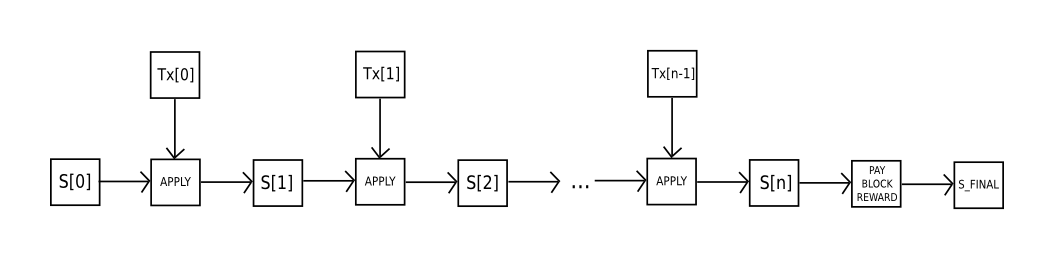
\includegraphics[width=0.9\linewidth]{../img/applyBlockDiagram}
	\caption{Minh hoạ thuật toán xác nhận khối cơ bản trong Ethereum}
	\label{fig:applyblockdiagram}
\end{figure}

Chuỗi khối của Ethereum có nhiều điểm tương tự như của Bitcoin, tuy nhiên có một số khác biệt sau: Khối Ethereum chứa một bản sao của cả danh sách giao dịch và trạng thái gần nhất. Bên cạnh đó, số khối và độ khó cũng được lưu trữ trong khối. Thuật toán xác nhận khối cơ bản trong Ethereum như sau:
\begin{itemize}
	\item Kiểm tra tham chiếu khối trước đó tồn tại và hợp lệ không.
	\item Kiểm tra dấu thời gian (timestamp) của khối lớn hơn dấu thời gian của khối được tham chiếu trước đó và nhỏ hơn 15 phút trong tương lai không.
	\item Kiểm tra số khối, độ khó, gốc giao dịch, gốc cha chú (uncle) và giới hạn gas là hợp lệ không.
	\item Kiểm tra xem chứng minh công việc (proof of work) trên khối là hợp lệ không.
	\item Đặt S[0] là trạng thái cuối ở khối trước đó.
	\item Đặt TX là danh sách giao dịch của khối, với n giao dịch. Đối với tất cả i từ 0...n-1, đặt S[i+1] = APPLY(S[i],TX[i]). Nếu bất kỳ ứng dụng nào trả về lỗi hoặc nếu tổng lượng gas tiêu thụ trong khối cho đến thời điểm này vượt quá GASLIMIT thì trả lại lỗi. (APPLY là một hàm thay đổi trạng thái S khi có giao dịch).
	\item Đặt S_FINAL là S[n], nhưng thêm phần thưởng cho thợ mỏ.
	\item Kiểm tra gốc cây Merkle của trạng thái S_FINAL có bằng với gốc trạng thái cuối cùng được cung cấp trong tiêu đề khối không. Nếu có, khối này là hợp lệ; Nếu không, nó không hợp lệ.
\end{itemize}

Cách tiếp cận có thể có vẻ không hiệu quả ở cái nhìn đầu tiên, bởi vì nó cần phải lưu trữ toàn bộ trạng thái với mỗi khối, nhưng hiệu quả thực tế là ngang với Bitcoin. Lý do là trạng thái được lưu trữ trong cấu trúc cây, và sau mỗi khối thì chỉ cần một phần nhỏ của cây phải thay đổi. Do đó, nói chung, giữa hai khối liền kề, phần lớn cây giống nhau, và vì vậy dữ liệu có thể được lưu trữ một lần và được tham chiếu hai lần bằng cách sử dụng các con trỏ (ví dụ: băm (hash) các cây con).

Một loại cây đặc biệt được gọi là "cây Patricia" được sử dụng để thực hiện việc này, bao gồm sửa đổi khái niệm cây Merkle cho phép chèn và xóa các nút một cách hiệu quả. Ngoài ra, vì tất cả các thông tin trạng thái là một phần của khối cuối cùng nên không cần lưu trữ toàn bộ lịch sử chuỗi khối đối với các nút không có khả năng lưu trữ nhiều.

\subsubsection{Solidity}
\begin{figure}[ht]
	\centering
	
\includegraphics[width=0.1\linewidth]{../img/logoSolidity}
	\caption{Logo Solidity}
	\label{fig:logosolidity}
\end{figure}

Solidity là một ngôn ngữ lập trình sử dụng để viết các chương trình hợp đồng thông minh, thứ mà sẽ được chạy trên EVM. Ngôn ngữ mới này là một sự pha trộn các quy ước từ mạng, hợp ngữ và phát triển web. 

Solidity là một ngôn ngữ hướng hợp đồng (contract-oriented) bậc cao, có cú pháp tương tự như ngôn ngữ C và JavaScript. Nó cho phép bạn phát triển hợp đồng và biên dịch sang mã EVM. Hiện nay nó là ngôn ngữ hàng đầu của Ethereum. Mặc dù nó ngôn ngữ phổ biến nhất để viết cho Ethereum nhưng nó không phải là ngôn ngữ đầu tiên và có lẽ cũng sẽ không phải ngôn ngữ cuối cùng.

Ngôn ngữ Solidity định kiểu mạnh, hỗ trợ thừa kế, thư viện và kiểu định nghĩa người dùng phức tạp cùng với các tính năng khác.

\subsubsection{Ứng dụng phi tập trung}
Ứng dụng phi tập trung (Decentralized App, viết tắt là DApp) là ứng dụng mã nguồn mở hoàn chỉnh, hoạt động độc lập, không có thực thể nào kiểm soát phần lớn các tokens của ứng dụng này. Dữ liệu và hồ sơ hoạt động của ứng dụng phải được lưu trữ dưới dạng mã hoá công khai, phân quyền chuỗi khối.

Ứng dụng này tạo các mã thông báo thông qua thuật toán theo một tiêu chuẩn hoặc bộ tiêu chuẩn và có thể phân phối một số hoặc tất cả các tokens của nó khi bắt đầu hoạt động. Các tokens này cần thiết cho việc sử dụng ứng dụng và bất kỳ đóng góp nào từ người dùng sẽ được thưởng bằng các khoản thanh toán trong các tokens của ứng dụng. Ứng dụng có thể thích ứng các giao thức của nó để đáp ứng với những cải tiến đề xuất và phản hồi thị trường nhưng tất cả thay đổi phải được quyết định bởi sự đồng thuận của người sử dụng. DApp rất có giá trị và có khả năng sẽ phá vỡ một số ngành công nghiệp.

Phân loại DApp:
\begin{itemize}
	\item Các ứng dụng phân cấp có chuỗi khối riêng như bitcoin.
	\item Giống như loại 1 nhưng có thêm token và các giao thức cần thiết như giao thức omni
	\item Giống như loại 2 nhưng có các mã thông báo cần thiết
\end{itemize}

Lợi ích của DApp:
\begin{itemize}
	\item The Safe Network: có sự bảo mật lớn nhất
	\item Factom: đơn giản hóa quá trình tăng cường quá trình ghi lại quá trình quản lý dữ liệu lớn
	\item BURST: giải quyết các vấn đề đã làm lưu trữ đám mây đắt đỏ và không đáng tin cậy
	\item Augur: được biết đến như là một thị trường dự đoán phân quyền để thưởng cho người sử dụng về các sự kiện dự báo
	\item BlockAuth: cung cấp một hệ thống đa chữ ký để chia sẻ dữ liệu cá nhân với các bên thứ ba
\end{itemize}

\subsubsection{Sự đồng thuận về việc chấp nhận khối}
Trên một mạng ngang hàng, mọi dữ liệu ở các nút cục bộ đều có thể bị thay đổi túy ý bởi người sở hữu nút đó và khi thực hiện nhân bản thì sẽ có các xung đột và ta khó có thể xác định đâu mới là chuỗi khối đúng. Vì vậy, để đảm bảo sự tin cậy của mạng cũng như chuỗi khối, ta phải có các cơ chế để làm sao tất các nút trên mạng đều đồng thuận khối thêm vào chuỗi đó là khối hợp lệ và sẽ phát hiện ra các hành vi phá hoại mạng bằng cách đưa vào các khối giả. Nói về cơ chế đồng thuận này thì hiện nay phổ biến nhất sẽ có hai cơ chế là chứng nhận công việc (Proof Of Work - POW) và chứng nhận cổ phần (Proof Of Stake - POS). Ngoài ra còn mô hình chứng nhận thẩm quyền (Proof Of Authority - POA) nhưng trước hết ta sẽ đi vào giải thích POW và POS.
\paragraph{POW}\mbox{}\\

Ta đã quá quen thuộc với việc các thợ mỏ mua các cỗ máy đắt tiền (gồm nhiều card đồ họa) để về đào coin. Việc này chúng tỏ họ đang tham gia vào một mạng lưới tiền ảo sử dụng mô hình POW. POW là một trong các cách để xác định sự đồng thuận của cộng đồng. Ở mô hình hay giải thuật này, để thêm mới một khối và blockchain đồi hỏi phải thực hiện các hàm tính toán rất phức tạp để tạo nên một giá trị băm hợp lệ (khó để tạo ra nhưng rất dễ dàng để xác định nó hợp lệ). Việc giải mã này ngoài việc cần những cấu hình mạnh còn tiêu tốn rất rất nhiều điện năng và gây nguy hại đến môi trường. Cộng đồng sẽ công nhận khối anh tạo ra dựa vào lượng công việc anh đã thực hiện được. Một yếu tố đặc trưng của mô hình này đó là sự xuất hiện của các khối dư thừa (orphan block) do có nhiều người tham gia cùng tạo nên một khối nên sẽ có trường hợp hai người tạo ra hai khối đều hợp lệ nhưng ta chỉ có thể chọn khối đến trước và khối kia (tốn rất nhiều năng lượng tạo ra) bị lãng phí và bỏ đi. Những đặc trưng kể trên phần nào nói lên nhược điểm của giải thuật mà phần lớn các đồng tiền ảo đang sử dụng

Khi độ khó để tạo ra một khối càng ngày càng tăng lên, việc đào ra một khối của các thợ mỏ ngày càng thấp và họ bắt đầu thua lỗ,một số sẽ quyết định từ bỏ hoặc tham gia vào các bể đào (mining pool). Việc này tạo ra các cỗ máy tập trung (trái với các tính chất phân tán mà mô hình mong muốn). Và còn một vấn đề hệ quả nữa là tấn công 51\% (51\% attack) sẽ được nên ở sau.

Nhưng nó phổ biến có nguyên nhân của nó. Giá trị sử dụng của nó là khi một đồng tiền ảo mới được phát hành, lượng tiền chưa được nhiều. Hầu hết các đồng tiền ảo sẽ chọn mô hình này để gia tăng lượng tiền mà vẫn kiểm soát được phần nào lạm phát của nó (điều mà ETH đã làm), tiền chỉ được tạo ra không hề dễ dàng.
\paragraph{POS}\mbox{}\\

Khi mà POW bộc lộ rõ các yếu điểm thì là lúc các mô hình và các giải thuật khác được đề xuất, trong đó có POS. Thực tế thì POS đã được áp dụng ở một số đồng tiền ảo, tiên phong trong đó là PeerCoin và Ethereum sẽ là cái tên tiếp theo áp dụng mô hình này. Mô hình POS thay vì công nhận công việc của anh bằng sức lực anh bỏ ra (chi cho phần cứng và năng lượng) thì lại công nhận bằng nó bằng cổ phần hay số tiền mà anh đặt cọc vào mỗi khối người đó sinh ra. Và giờ đây, mỗi khối không phải là cuộc chạy đua xem ai giải mã được chính xác và nhanh nhất (có thể gây lãng phí với các khối thừa) mà việc tạo khối được chỉ định cho người nào góp cổ phần nhiều nhất vì hệ thống tự động hiểu rằng nếu anh góp vào nhiều tiền như vậy thì anh cũng sẽ có đủ khả năng tính toán để tạo ra khối mới.Và một điều quan trọng nữa là sẽ không còn tồn tại việc thưởng ETH theo mỗi khối đào được mà chỉ trả cho người tạo khối một khoản tiền vì đã thực hiện giao dịch (transaction fee).

Việc sử dụng POS sẽ dẫn đến các lợi ích như sau. Tiết kiệm năng lượng, giúp mạng lưới phân tán hơn, giúp đảm bảo lợi ích người đào.

\paragraph{POA}\mbox{}\\

POA khá khác so với hai mô hình đồng thuận trước, trong khi hai mô hình trên vẫn giữ tính ẩn danh của tất cả những người tham gia và sự tin tưởng khó có thể đạt tới sự chắc chắn (tạm tin tưởng vào lượng công việc cũng như cổ phần) thì thay vào đó ta sẽ có các cơ quan được chứng thực một cách hợp pháp và công khai tham gia vào mạng như các thành viên kiểm chứng. Những cơ quan này sẽ sở hữu các tài khoản và các nút được coi là có thẩm quyền, các thành viên trong mạng có thể tin tưởng hoàn toàn họ và họ sẽ đóng vai trò chính trong việc kiểm tra các giao dịch và các khối có hợp lệ hay không. Mạng theo mô hình này sẽ có một số lợi thế vượt trội so với hai mô hình kia như thời gian tạo khối tương đối ngắn, không lãng phí vì không cần phải đào, giúp cải thiện thời gian triển khai, kiểm thử và ngăn chặn các cuộc tấn công spam. Ethereum đã triển khai một mạng thử nghiệm triển khai mô hình này có tên là Kovan, bạn có thể xem chi tiết hơn tại \url{https://github.com/kovan-testnet/proposal}.

\subsubsection{Whisper và Swarm}
Các ứng dụng tại máy chủ hiện nay thường sẽ thưc hiện ba việc chính sau: tính toán để đưa ra câu trả lời, lưu trữ dữ liệu phản hồi lại tức thì các cử chỉ của người dùng (ứng dụng thời gian thực). Xét lại nền tảng Ethereum chúng ta thấy đã có nền tảng tính toán là máy ảo Ethereum thực hiện nhưng hai thành phần còn lại vẫn chưa hỗ trợ. Các nhà lập trình của Ethereum đã thấy điều đó và họ đã và đang phát triển hai thành phần đó trong các phiên bản tiếp theo của Ethereum. Từ đó ta có các thành phần như sau:
\begin{itemize}
	\item EVM: Máy trạng thái phi tập trung
	\item Swarm: Lưu trữ phi tập trung
	\item Whisper: Gửi tin nhắn phi tập trung
\end{itemize}

\paragraph{Whisper}\mbox{}\\

Whisper là một hệ thống nhắn tin phi tập trung, là một phần của giao thức Ethereum và sẽ sẵn có cho các ứng dụng web sử dụng EVM cho phần backend. Không giống với cách thông thường là mọi thay đổi đều được lưu ở chuỗi khối, dữ liệu của mỗi tin nhắn sẽ được truyền trực tiếp giữa các hợp đồng thông minh với nhau.

\paragraph{Swarm}\mbox{}\\

Swarm là giao thức dành cho các dữ liệu được đánh địa chỉ. Nó họạt động với dữ liệu bất biến, phân mảnh (sharding) nó và lưu trữ nó trong mạng phân tán và có thể dễ dàng gọi nó nếu ứng dụng cần. Mục tiêu của Swarm là có thể tìm các phiên bản khác nhau của dữ liệu của một tệp ở cùng một địa chỉ, làm theo hệ phân cấp như các URL hiện nay, tức là có cấu trúc thư mục.

Chính Swarm có thể hiện thực hóa việc đưa một ứng dụng web đơn giản triển khai hoàn toàn trên nền tảng phi tập trung với các tệp HTML, CSS, JS được lưu lại và trả về nếu có yêu cầu từ người dùng. Nó sẽ thực sự khác biệt khi ứng dụng web của bạn vươn tới một thứ được gọi là trực tuyến 100\% thực sự chứ không phải là 99.99\% như hiện tại. Tất nhiên chặng đường vẫn còn xa nhưng thực sự đáng kỳ vọng cho một ứng dụng web như vậy.